%*----------- SLIDE -------------------------------------------------------------
\begin{frame}[t]{A pesquisa na vida real} 
    \transdissolve[duration=0.5]
    A complexidade do conhecimento nas inovações tem aumentado ano após ano. A necessidade do ser humano em alcançar patamares cada vez mais eficientes em nosso dia a dia, faz com que tenhamos cada vez mais uma capacidade de otimização na busca por conhecimento.

    \centering
    \vspace*{0.1cm}
    \Large{O tempo é vital.}

    \roundpic[xshift=0cm,yshift=0cm]{4cm}{7cm}{time}
    %\newline

        % \begin{columns}[t]
        %     \column{.05\linewidth}
        %     \column{.4\linewidth}
        %         \huge{O tempo é vital.}
        %     \column{.6\linewidth}
        %     \begin{center}
        %     %\centerline{
        %         \begin{figure}
        %             %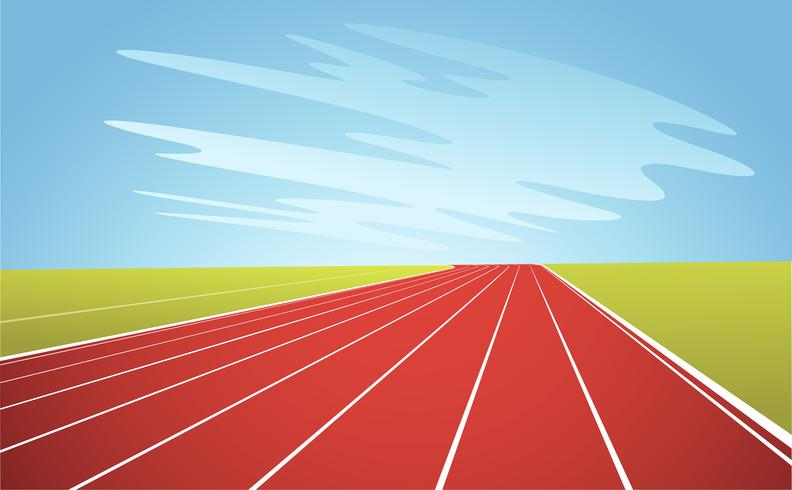
\includegraphics[width=1\textwidth]{pista}
        %             %\caption{Pista de corrida \cite{agostini2007}}
        %             \roundpic[xshift=0cm,yshift=0cm]{4cm}{7cm}{time}
        %             %\caption{Pista de corrida \cite{agostini2007}}
        %         \end{figure}
        %     %}
        %     \end{center}
        % \end{columns}
%*----------- notes
    \note[item]{Notes can help you to remember important information. Turn on the notes option.}
\end{frame}
%-
%*----------- SLIDE -------------------------------------------------------------
\begin{frame}[c]{Como vocês realizam as buscas por artigos?} 
    \transdissolve[duration=0.5]
   
    \begin{center}
        \Wider{%
        \begin{shaded}
        \begin{center}
            \vspace*{0.5cm}
            \resizebox{!}{0.7cm}{%
                \textcolor{cyan}{G}\textcolor{red}{o}\textcolor{orange}{o}\textcolor{cyan}{g}\textcolor{teal}{l}\textcolor{red}{e}?
            }%
        \end{center}
        \end{shaded}
        }%
    \end{center}
%*----------- notes
    \note[item]{Notes can help you to remember important information. Turn on the notes option.}
\end{frame}
%-
%*----------- SLIDE -------------------------------------------------------------
\begin{frame}[c]{Como vocês realizam as buscas por artigos?} 
    \transdissolve[duration=0.5]
   
    \centering
    
\includegraphics[clip, trim = 0 0 0 0,  width=.83\textwidth]{databases.jpg}
%*----------- notes
    \note[item]{Notes can help you to remember important information. Turn on the notes option.}
\end{frame}
%-
%*----------- SLIDE -------------------------------------------------------------
\begin{frame}[c]{Como vocês realizam as buscas por artigos?} 
    \framesubtitle{Pouco tempo para muito resultado}
    \transdissolve[duration=0.5]
   
    \centering
    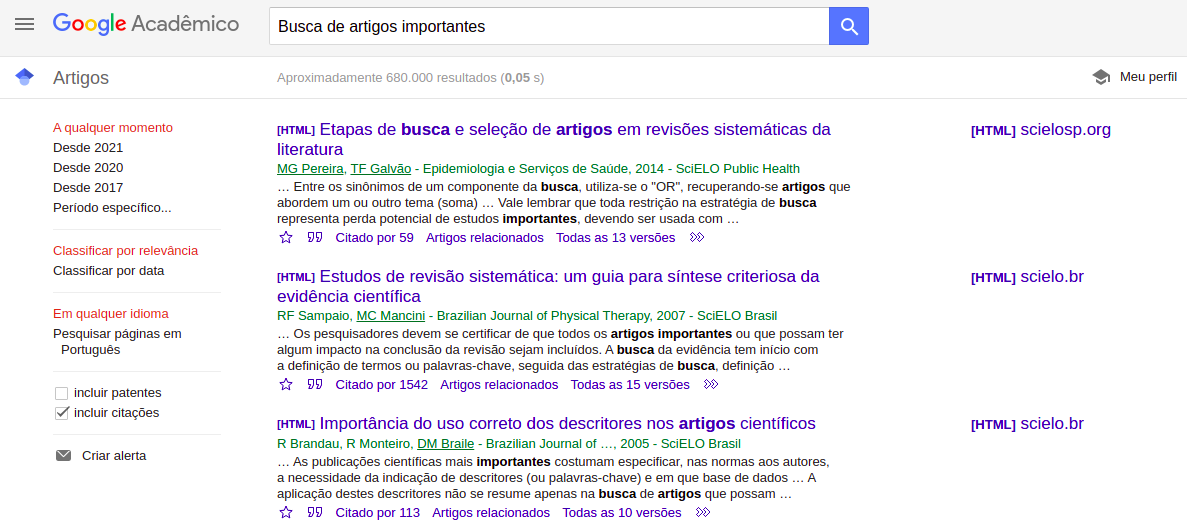
\includegraphics[clip, trim = 0 0 0 0,  width=1\textwidth]{googleacademico2.png}
%*----------- notes
    \note[item]{Notes can help you to remember important information. Turn on the notes option.}
\end{frame}
%-
%*----------- SLIDE -------------------------------------------------------------
\begin{frame}[c]{Como vocês realizam as buscas por artigos?} 
    \framesubtitle{Pouco tempo para muito resultado}
    \transdissolve[duration=0.5]
   
    \centering
    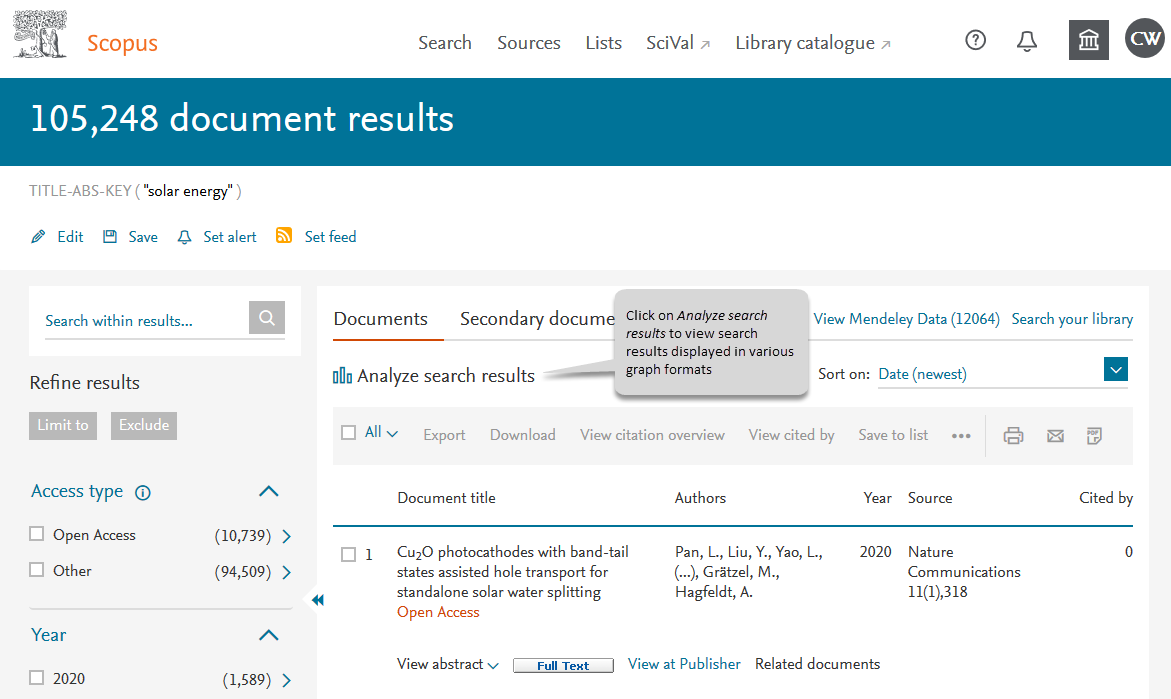
\includegraphics[clip, trim = 0 0 0 0,  width=.75\textwidth]{scopus.png}
%*----------- notes
    \note[item]{Notes can help you to remember important information. Turn on the notes option.}
\end{frame}
%-
%*----------- SLIDE -------------------------------------------------------------
\begin{frame}[c]{Como vocês realizam as buscas por artigos?} 
    \framesubtitle{Pouco tempo para muito resultado}
    \transdissolve[duration=0.5]
   
    \centering
    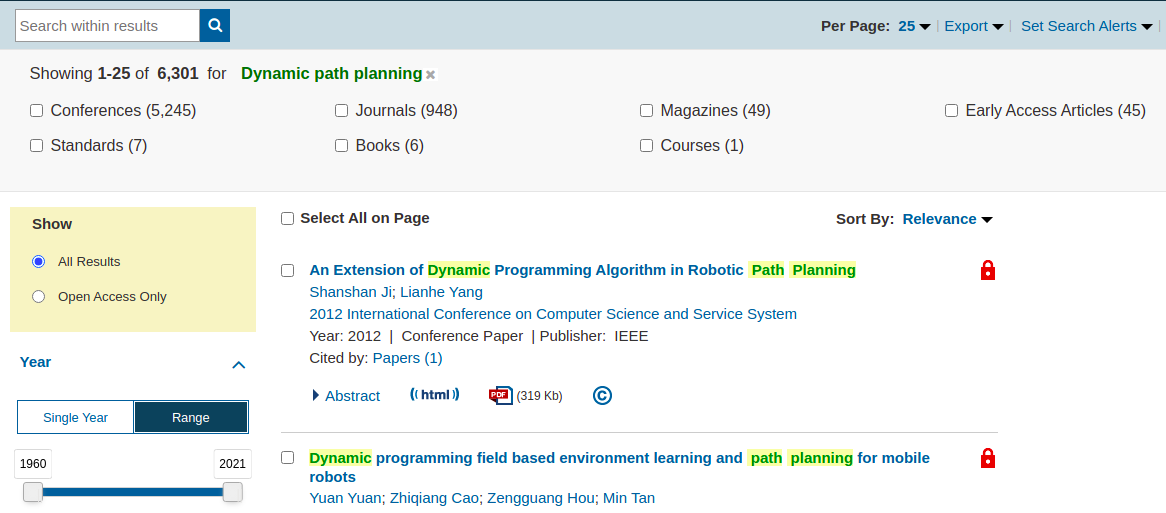
\includegraphics[clip, trim = 0 0 0 0,  width=1\textwidth]{ieee.png}
%*----------- notes
    \note[item]{Notes can help you to remember important information. Turn on the notes option.}
\end{frame}
%-
%*----------- SLIDE -------------------------------------------------------------
\begin{frame}[t]{Tempo e precisão}
    \transboxout[duration=0.5]
    %\framesubtitle{Darwin-OP}
    Uma das vertentes da tecnologia é a capacidade de tornar os processos mais rápidos e precisos, suportando a vida humana no planeta.

    \vspace*{0.2cm}
    Alguns fatores impulsionadores
		\begin{itemize}
			\item Competitividade
			\item Prazo de entrega
			\item Concluir um trabalho 
		\end{itemize}

    \vspace*{0.2cm}
    
\includegraphics[clip, trim = 0 420 0 80, width=1\textwidth]{time-and-precision.jpeg}

    \begin{columns}
        \column{.1\textwidth}
        \column{.5\textwidth}
        \column{.4\textwidth}
    \end{columns}
%*----------- notes
    \note[item]{Notes can help you to remember important information. Turn on the notes option.}
\end{frame}
%-
